% Created by tikzDevice version 0.12.3 on 2020-03-23 21:28:04
% !TEX encoding = UTF-8 Unicode
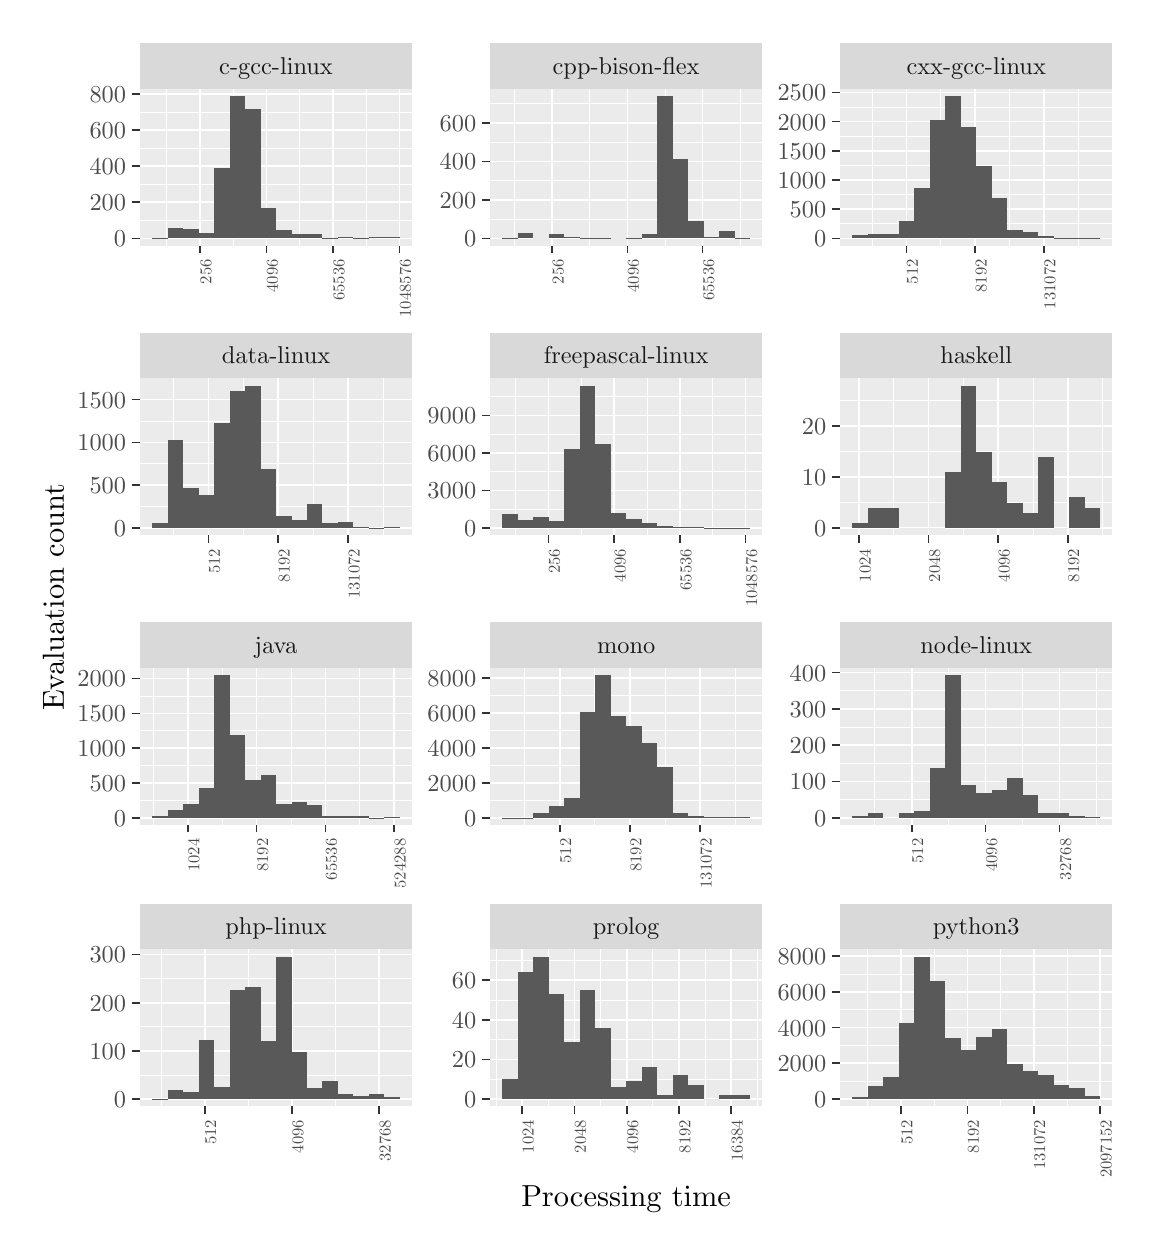
\begin{tikzpicture}[x=1pt,y=1pt]
\definecolor{fillColor}{RGB}{255,255,255}
\path[use as bounding box,fill=fillColor,fill opacity=0.00] (0,0) rectangle (397.48,433.62);
\begin{scope}
\path[clip] (  0.00,  0.00) rectangle (397.48,433.62);
\definecolor{drawColor}{RGB}{255,255,255}
\definecolor{fillColor}{RGB}{255,255,255}

\path[draw=drawColor,line width= 0.6pt,line join=round,line cap=round,fill=fillColor] (  0.00,  0.00) rectangle (397.48,433.62);
\end{scope}
\begin{scope}
\path[clip] ( 40.51,354.90) rectangle (138.97,411.55);
\definecolor{fillColor}{gray}{0.92}

\path[fill=fillColor] ( 40.51,354.90) rectangle (138.97,411.55);
\definecolor{drawColor}{RGB}{255,255,255}

\path[draw=drawColor,line width= 0.3pt,line join=round] ( 40.51,364.00) --
	(138.97,364.00);

\path[draw=drawColor,line width= 0.3pt,line join=round] ( 40.51,377.06) --
	(138.97,377.06);

\path[draw=drawColor,line width= 0.3pt,line join=round] ( 40.51,390.11) --
	(138.97,390.11);

\path[draw=drawColor,line width= 0.3pt,line join=round] ( 40.51,403.16) --
	(138.97,403.16);

\path[draw=drawColor,line width= 0.3pt,line join=round] ( 50.26,354.90) --
	( 50.26,411.55);

\path[draw=drawColor,line width= 0.3pt,line join=round] ( 74.29,354.90) --
	( 74.29,411.55);

\path[draw=drawColor,line width= 0.3pt,line join=round] ( 98.32,354.90) --
	( 98.32,411.55);

\path[draw=drawColor,line width= 0.3pt,line join=round] (122.34,354.90) --
	(122.34,411.55);

\path[draw=drawColor,line width= 0.6pt,line join=round] ( 40.51,357.48) --
	(138.97,357.48);

\path[draw=drawColor,line width= 0.6pt,line join=round] ( 40.51,370.53) --
	(138.97,370.53);

\path[draw=drawColor,line width= 0.6pt,line join=round] ( 40.51,383.58) --
	(138.97,383.58);

\path[draw=drawColor,line width= 0.6pt,line join=round] ( 40.51,396.64) --
	(138.97,396.64);

\path[draw=drawColor,line width= 0.6pt,line join=round] ( 40.51,409.69) --
	(138.97,409.69);

\path[draw=drawColor,line width= 0.6pt,line join=round] ( 62.27,354.90) --
	( 62.27,411.55);

\path[draw=drawColor,line width= 0.6pt,line join=round] ( 86.30,354.90) --
	( 86.30,411.55);

\path[draw=drawColor,line width= 0.6pt,line join=round] (110.33,354.90) --
	(110.33,411.55);

\path[draw=drawColor,line width= 0.6pt,line join=round] (134.36,354.90) --
	(134.36,411.55);
\definecolor{fillColor}{gray}{0.35}

\path[fill=fillColor] ( 44.99,357.48) rectangle ( 50.58,357.74);

\path[fill=fillColor] ( 50.58,357.48) rectangle ( 56.17,361.20);

\path[fill=fillColor] ( 56.17,357.48) rectangle ( 61.77,360.87);

\path[fill=fillColor] ( 61.77,357.48) rectangle ( 67.36,359.30);

\path[fill=fillColor] ( 67.36,357.48) rectangle ( 72.96,382.80);

\path[fill=fillColor] ( 72.96,357.48) rectangle ( 78.55,408.97);

\path[fill=fillColor] ( 78.55,357.48) rectangle ( 84.15,404.34);

\path[fill=fillColor] ( 84.15,357.48) rectangle ( 89.74,368.44);

\path[fill=fillColor] ( 89.74,357.48) rectangle ( 95.34,360.41);

\path[fill=fillColor] ( 95.34,357.48) rectangle (100.93,359.04);

\path[fill=fillColor] (100.93,357.48) rectangle (106.52,358.91);

\path[fill=fillColor] (106.52,357.48) rectangle (112.12,357.67);

\path[fill=fillColor] (112.12,357.48) rectangle (117.71,358.00);

\path[fill=fillColor] (117.71,357.48) rectangle (123.31,357.74);

\path[fill=fillColor] (123.31,357.48) rectangle (128.90,357.80);

\path[fill=fillColor] (128.90,357.48) rectangle (134.50,358.00);
\end{scope}
\begin{scope}
\path[clip] ( 40.51,250.24) rectangle (138.97,306.88);
\definecolor{fillColor}{gray}{0.92}

\path[fill=fillColor] ( 40.51,250.24) rectangle (138.97,306.88);
\definecolor{drawColor}{RGB}{255,255,255}

\path[draw=drawColor,line width= 0.3pt,line join=round] ( 40.51,260.54) --
	(138.97,260.54);

\path[draw=drawColor,line width= 0.3pt,line join=round] ( 40.51,276.01) --
	(138.97,276.01);

\path[draw=drawColor,line width= 0.3pt,line join=round] ( 40.51,291.47) --
	(138.97,291.47);

\path[draw=drawColor,line width= 0.3pt,line join=round] ( 52.75,250.24) --
	( 52.75,306.88);

\path[draw=drawColor,line width= 0.3pt,line join=round] ( 77.96,250.24) --
	( 77.96,306.88);

\path[draw=drawColor,line width= 0.3pt,line join=round] (103.17,250.24) --
	(103.17,306.88);

\path[draw=drawColor,line width= 0.3pt,line join=round] (128.39,250.24) --
	(128.39,306.88);

\path[draw=drawColor,line width= 0.6pt,line join=round] ( 40.51,252.81) --
	(138.97,252.81);

\path[draw=drawColor,line width= 0.6pt,line join=round] ( 40.51,268.28) --
	(138.97,268.28);

\path[draw=drawColor,line width= 0.6pt,line join=round] ( 40.51,283.74) --
	(138.97,283.74);

\path[draw=drawColor,line width= 0.6pt,line join=round] ( 40.51,299.21) --
	(138.97,299.21);

\path[draw=drawColor,line width= 0.6pt,line join=round] ( 65.35,250.24) --
	( 65.35,306.88);

\path[draw=drawColor,line width= 0.6pt,line join=round] ( 90.57,250.24) --
	( 90.57,306.88);

\path[draw=drawColor,line width= 0.6pt,line join=round] (115.78,250.24) --
	(115.78,306.88);
\definecolor{fillColor}{gray}{0.35}

\path[fill=fillColor] ( 44.99,252.81) rectangle ( 50.58,254.51);

\path[fill=fillColor] ( 50.58,252.81) rectangle ( 56.17,284.52);

\path[fill=fillColor] ( 56.17,252.81) rectangle ( 61.77,267.10);

\path[fill=fillColor] ( 61.77,252.81) rectangle ( 67.36,264.72);

\path[fill=fillColor] ( 67.36,252.81) rectangle ( 72.96,290.61);

\path[fill=fillColor] ( 72.96,252.81) rectangle ( 78.55,302.33);

\path[fill=fillColor] ( 78.55,252.81) rectangle ( 84.15,304.31);

\path[fill=fillColor] ( 84.15,252.81) rectangle ( 89.74,274.06);

\path[fill=fillColor] ( 89.74,252.81) rectangle ( 95.34,257.27);

\path[fill=fillColor] ( 95.34,252.81) rectangle (100.93,255.84);

\path[fill=fillColor] (100.93,252.81) rectangle (106.52,261.41);

\path[fill=fillColor] (106.52,252.81) rectangle (112.12,254.45);

\path[fill=fillColor] (112.12,252.81) rectangle (117.71,254.95);

\path[fill=fillColor] (117.71,252.81) rectangle (123.31,253.15);

\path[fill=fillColor] (123.31,252.81) rectangle (128.90,252.97);

\path[fill=fillColor] (128.90,252.81) rectangle (134.50,253.31);
\end{scope}
\begin{scope}
\path[clip] ( 40.51,145.57) rectangle (138.97,202.22);
\definecolor{fillColor}{gray}{0.92}

\path[fill=fillColor] ( 40.51,145.57) rectangle (138.97,202.22);
\definecolor{drawColor}{RGB}{255,255,255}

\path[draw=drawColor,line width= 0.3pt,line join=round] ( 40.51,154.43) --
	(138.97,154.43);

\path[draw=drawColor,line width= 0.3pt,line join=round] ( 40.51,167.00) --
	(138.97,167.00);

\path[draw=drawColor,line width= 0.3pt,line join=round] ( 40.51,179.56) --
	(138.97,179.56);

\path[draw=drawColor,line width= 0.3pt,line join=round] ( 40.51,192.13) --
	(138.97,192.13);

\path[draw=drawColor,line width= 0.3pt,line join=round] ( 45.46,145.57) --
	( 45.46,202.22);

\path[draw=drawColor,line width= 0.3pt,line join=round] ( 70.30,145.57) --
	( 70.30,202.22);

\path[draw=drawColor,line width= 0.3pt,line join=round] ( 95.15,145.57) --
	( 95.15,202.22);

\path[draw=drawColor,line width= 0.3pt,line join=round] (120.00,145.57) --
	(120.00,202.22);

\path[draw=drawColor,line width= 0.6pt,line join=round] ( 40.51,148.15) --
	(138.97,148.15);

\path[draw=drawColor,line width= 0.6pt,line join=round] ( 40.51,160.72) --
	(138.97,160.72);

\path[draw=drawColor,line width= 0.6pt,line join=round] ( 40.51,173.28) --
	(138.97,173.28);

\path[draw=drawColor,line width= 0.6pt,line join=round] ( 40.51,185.85) --
	(138.97,185.85);

\path[draw=drawColor,line width= 0.6pt,line join=round] ( 40.51,198.41) --
	(138.97,198.41);

\path[draw=drawColor,line width= 0.6pt,line join=round] ( 57.88,145.57) --
	( 57.88,202.22);

\path[draw=drawColor,line width= 0.6pt,line join=round] ( 82.73,145.57) --
	( 82.73,202.22);

\path[draw=drawColor,line width= 0.6pt,line join=round] (107.57,145.57) --
	(107.57,202.22);

\path[draw=drawColor,line width= 0.6pt,line join=round] (132.42,145.57) --
	(132.42,202.22);
\definecolor{fillColor}{gray}{0.35}

\path[fill=fillColor] ( 44.99,148.15) rectangle ( 50.58,148.80);

\path[fill=fillColor] ( 50.58,148.15) rectangle ( 56.17,150.89);

\path[fill=fillColor] ( 56.17,148.15) rectangle ( 61.77,153.13);

\path[fill=fillColor] ( 61.77,148.15) rectangle ( 67.36,158.83);

\path[fill=fillColor] ( 67.36,148.15) rectangle ( 72.96,199.65);

\path[fill=fillColor] ( 72.96,148.15) rectangle ( 78.55,178.11);

\path[fill=fillColor] ( 78.55,148.15) rectangle ( 84.15,161.75);

\path[fill=fillColor] ( 84.15,148.15) rectangle ( 89.74,163.48);

\path[fill=fillColor] ( 89.74,148.15) rectangle ( 95.34,153.23);

\path[fill=fillColor] ( 95.34,148.15) rectangle (100.93,153.70);

\path[fill=fillColor] (100.93,148.15) rectangle (106.52,152.77);

\path[fill=fillColor] (106.52,148.15) rectangle (112.12,148.78);

\path[fill=fillColor] (112.12,148.15) rectangle (117.71,148.80);

\path[fill=fillColor] (117.71,148.15) rectangle (123.31,148.60);

\path[fill=fillColor] (123.31,148.15) rectangle (128.90,148.17);

\path[fill=fillColor] (128.90,148.15) rectangle (134.50,148.27);
\end{scope}
\begin{scope}
\path[clip] ( 40.51, 43.91) rectangle (138.97,100.56);
\definecolor{fillColor}{gray}{0.92}

\path[fill=fillColor] ( 40.51, 43.91) rectangle (138.97,100.56);
\definecolor{drawColor}{RGB}{255,255,255}

\path[draw=drawColor,line width= 0.3pt,line join=round] ( 40.51, 55.18) --
	(138.97, 55.18);

\path[draw=drawColor,line width= 0.3pt,line join=round] ( 40.51, 72.58) --
	(138.97, 72.58);

\path[draw=drawColor,line width= 0.3pt,line join=round] ( 40.51, 89.98) --
	(138.97, 89.98);

\path[draw=drawColor,line width= 0.3pt,line join=round] ( 48.25, 43.91) --
	( 48.25,100.56);

\path[draw=drawColor,line width= 0.3pt,line join=round] ( 79.77, 43.91) --
	( 79.77,100.56);

\path[draw=drawColor,line width= 0.3pt,line join=round] (111.28, 43.91) --
	(111.28,100.56);

\path[draw=drawColor,line width= 0.6pt,line join=round] ( 40.51, 46.48) --
	(138.97, 46.48);

\path[draw=drawColor,line width= 0.6pt,line join=round] ( 40.51, 63.88) --
	(138.97, 63.88);

\path[draw=drawColor,line width= 0.6pt,line join=round] ( 40.51, 81.28) --
	(138.97, 81.28);

\path[draw=drawColor,line width= 0.6pt,line join=round] ( 40.51, 98.68) --
	(138.97, 98.68);

\path[draw=drawColor,line width= 0.6pt,line join=round] ( 64.01, 43.91) --
	( 64.01,100.56);

\path[draw=drawColor,line width= 0.6pt,line join=round] ( 95.52, 43.91) --
	( 95.52,100.56);

\path[draw=drawColor,line width= 0.6pt,line join=round] (127.04, 43.91) --
	(127.04,100.56);
\definecolor{fillColor}{gray}{0.35}

\path[fill=fillColor] ( 44.99, 46.48) rectangle ( 50.58, 46.66);

\path[fill=fillColor] ( 50.58, 46.48) rectangle ( 56.17, 49.79);

\path[fill=fillColor] ( 56.17, 46.48) rectangle ( 61.77, 49.09);

\path[fill=fillColor] ( 61.77, 46.48) rectangle ( 67.36, 67.71);

\path[fill=fillColor] ( 67.36, 46.48) rectangle ( 72.96, 51.01);

\path[fill=fillColor] ( 72.96, 46.48) rectangle ( 78.55, 85.98);

\path[fill=fillColor] ( 78.55, 46.48) rectangle ( 84.15, 86.85);

\path[fill=fillColor] ( 84.15, 46.48) rectangle ( 89.74, 67.54);

\path[fill=fillColor] ( 89.74, 46.48) rectangle ( 95.34, 97.98);

\path[fill=fillColor] ( 95.34, 46.48) rectangle (100.93, 63.53);

\path[fill=fillColor] (100.93, 46.48) rectangle (106.52, 50.31);

\path[fill=fillColor] (106.52, 46.48) rectangle (112.12, 52.92);

\path[fill=fillColor] (112.12, 46.48) rectangle (117.71, 48.40);

\path[fill=fillColor] (117.71, 46.48) rectangle (123.31, 47.70);

\path[fill=fillColor] (123.31, 46.48) rectangle (128.90, 48.22);

\path[fill=fillColor] (128.90, 46.48) rectangle (134.50, 47.35);
\end{scope}
\begin{scope}
\path[clip] (167.02,354.90) rectangle (265.48,411.55);
\definecolor{fillColor}{gray}{0.92}

\path[fill=fillColor] (167.02,354.90) rectangle (265.48,411.55);
\definecolor{drawColor}{RGB}{255,255,255}

\path[draw=drawColor,line width= 0.3pt,line join=round] (167.02,364.44) --
	(265.48,364.44);

\path[draw=drawColor,line width= 0.3pt,line join=round] (167.02,378.35) --
	(265.48,378.35);

\path[draw=drawColor,line width= 0.3pt,line join=round] (167.02,392.27) --
	(265.48,392.27);

\path[draw=drawColor,line width= 0.3pt,line join=round] (167.02,406.19) --
	(265.48,406.19);

\path[draw=drawColor,line width= 0.3pt,line join=round] (175.92,354.90) --
	(175.92,411.55);

\path[draw=drawColor,line width= 0.3pt,line join=round] (203.11,354.90) --
	(203.11,411.55);

\path[draw=drawColor,line width= 0.3pt,line join=round] (230.30,354.90) --
	(230.30,411.55);

\path[draw=drawColor,line width= 0.3pt,line join=round] (257.49,354.90) --
	(257.49,411.55);

\path[draw=drawColor,line width= 0.6pt,line join=round] (167.02,357.48) --
	(265.48,357.48);

\path[draw=drawColor,line width= 0.6pt,line join=round] (167.02,371.39) --
	(265.48,371.39);

\path[draw=drawColor,line width= 0.6pt,line join=round] (167.02,385.31) --
	(265.48,385.31);

\path[draw=drawColor,line width= 0.6pt,line join=round] (167.02,399.23) --
	(265.48,399.23);

\path[draw=drawColor,line width= 0.6pt,line join=round] (189.51,354.90) --
	(189.51,411.55);

\path[draw=drawColor,line width= 0.6pt,line join=round] (216.70,354.90) --
	(216.70,411.55);

\path[draw=drawColor,line width= 0.6pt,line join=round] (243.89,354.90) --
	(243.89,411.55);
\definecolor{fillColor}{gray}{0.35}

\path[fill=fillColor] (171.49,357.48) rectangle (177.09,357.75);

\path[fill=fillColor] (177.09,357.48) rectangle (182.68,359.42);

\path[fill=fillColor] (182.68,357.48) rectangle (188.28,357.48);

\path[fill=fillColor] (188.28,357.48) rectangle (193.87,359.15);

\path[fill=fillColor] (193.87,357.48) rectangle (199.46,357.82);

\path[fill=fillColor] (199.46,357.48) rectangle (205.06,357.55);

\path[fill=fillColor] (205.06,357.48) rectangle (210.65,357.55);

\path[fill=fillColor] (210.65,357.48) rectangle (216.25,357.48);

\path[fill=fillColor] (216.25,357.48) rectangle (221.84,357.55);

\path[fill=fillColor] (221.84,357.48) rectangle (227.44,358.94);

\path[fill=fillColor] (227.44,357.48) rectangle (233.03,408.97);

\path[fill=fillColor] (233.03,357.48) rectangle (238.63,386.15);

\path[fill=fillColor] (238.63,357.48) rectangle (244.22,363.74);

\path[fill=fillColor] (244.22,357.48) rectangle (249.81,357.82);

\path[fill=fillColor] (249.81,357.48) rectangle (255.41,360.12);

\path[fill=fillColor] (255.41,357.48) rectangle (261.00,357.55);
\end{scope}
\begin{scope}
\path[clip] (167.02,250.24) rectangle (265.48,306.88);
\definecolor{fillColor}{gray}{0.92}

\path[fill=fillColor] (167.02,250.24) rectangle (265.48,306.88);
\definecolor{drawColor}{RGB}{255,255,255}

\path[draw=drawColor,line width= 0.3pt,line join=round] (167.02,259.60) --
	(265.48,259.60);

\path[draw=drawColor,line width= 0.3pt,line join=round] (167.02,273.17) --
	(265.48,273.17);

\path[draw=drawColor,line width= 0.3pt,line join=round] (167.02,286.75) --
	(265.48,286.75);

\path[draw=drawColor,line width= 0.3pt,line join=round] (167.02,300.32) --
	(265.48,300.32);

\path[draw=drawColor,line width= 0.3pt,line join=round] (176.34,250.24) --
	(176.34,306.88);

\path[draw=drawColor,line width= 0.3pt,line join=round] (200.08,250.24) --
	(200.08,306.88);

\path[draw=drawColor,line width= 0.3pt,line join=round] (223.82,250.24) --
	(223.82,306.88);

\path[draw=drawColor,line width= 0.3pt,line join=round] (247.57,250.24) --
	(247.57,306.88);

\path[draw=drawColor,line width= 0.6pt,line join=round] (167.02,252.81) --
	(265.48,252.81);

\path[draw=drawColor,line width= 0.6pt,line join=round] (167.02,266.39) --
	(265.48,266.39);

\path[draw=drawColor,line width= 0.6pt,line join=round] (167.02,279.96) --
	(265.48,279.96);

\path[draw=drawColor,line width= 0.6pt,line join=round] (167.02,293.53) --
	(265.48,293.53);

\path[draw=drawColor,line width= 0.6pt,line join=round] (188.21,250.24) --
	(188.21,306.88);

\path[draw=drawColor,line width= 0.6pt,line join=round] (211.95,250.24) --
	(211.95,306.88);

\path[draw=drawColor,line width= 0.6pt,line join=round] (235.70,250.24) --
	(235.70,306.88);

\path[draw=drawColor,line width= 0.6pt,line join=round] (259.44,250.24) --
	(259.44,306.88);
\definecolor{fillColor}{gray}{0.35}

\path[fill=fillColor] (171.49,252.81) rectangle (177.09,258.04);

\path[fill=fillColor] (177.09,252.81) rectangle (182.68,255.54);

\path[fill=fillColor] (182.68,252.81) rectangle (188.28,256.75);

\path[fill=fillColor] (188.28,252.81) rectangle (193.87,255.46);

\path[fill=fillColor] (193.87,252.81) rectangle (199.46,281.33);

\path[fill=fillColor] (199.46,252.81) rectangle (205.06,304.31);

\path[fill=fillColor] (205.06,252.81) rectangle (210.65,283.35);

\path[fill=fillColor] (210.65,252.81) rectangle (216.25,258.27);

\path[fill=fillColor] (216.25,252.81) rectangle (221.84,256.08);

\path[fill=fillColor] (221.84,252.81) rectangle (227.44,254.45);

\path[fill=fillColor] (227.44,252.81) rectangle (233.03,253.43);

\path[fill=fillColor] (233.03,252.81) rectangle (238.63,253.22);

\path[fill=fillColor] (238.63,252.81) rectangle (244.22,253.10);

\path[fill=fillColor] (244.22,252.81) rectangle (249.81,252.95);

\path[fill=fillColor] (249.81,252.81) rectangle (255.41,252.90);

\path[fill=fillColor] (255.41,252.81) rectangle (261.00,252.82);
\end{scope}
\begin{scope}
\path[clip] (167.02,145.57) rectangle (265.48,202.22);
\definecolor{fillColor}{gray}{0.92}

\path[fill=fillColor] (167.02,145.57) rectangle (265.48,202.22);
\definecolor{drawColor}{RGB}{255,255,255}

\path[draw=drawColor,line width= 0.3pt,line join=round] (167.02,154.46) --
	(265.48,154.46);

\path[draw=drawColor,line width= 0.3pt,line join=round] (167.02,167.08) --
	(265.48,167.08);

\path[draw=drawColor,line width= 0.3pt,line join=round] (167.02,179.70) --
	(265.48,179.70);

\path[draw=drawColor,line width= 0.3pt,line join=round] (167.02,192.33) --
	(265.48,192.33);

\path[draw=drawColor,line width= 0.3pt,line join=round] (179.55,145.57) --
	(179.55,202.22);

\path[draw=drawColor,line width= 0.3pt,line join=round] (204.93,145.57) --
	(204.93,202.22);

\path[draw=drawColor,line width= 0.3pt,line join=round] (230.31,145.57) --
	(230.31,202.22);

\path[draw=drawColor,line width= 0.3pt,line join=round] (255.69,145.57) --
	(255.69,202.22);

\path[draw=drawColor,line width= 0.6pt,line join=round] (167.02,148.15) --
	(265.48,148.15);

\path[draw=drawColor,line width= 0.6pt,line join=round] (167.02,160.77) --
	(265.48,160.77);

\path[draw=drawColor,line width= 0.6pt,line join=round] (167.02,173.39) --
	(265.48,173.39);

\path[draw=drawColor,line width= 0.6pt,line join=round] (167.02,186.01) --
	(265.48,186.01);

\path[draw=drawColor,line width= 0.6pt,line join=round] (167.02,198.64) --
	(265.48,198.64);

\path[draw=drawColor,line width= 0.6pt,line join=round] (192.24,145.57) --
	(192.24,202.22);

\path[draw=drawColor,line width= 0.6pt,line join=round] (217.62,145.57) --
	(217.62,202.22);

\path[draw=drawColor,line width= 0.6pt,line join=round] (243.00,145.57) --
	(243.00,202.22);
\definecolor{fillColor}{gray}{0.35}

\path[fill=fillColor] (171.49,148.15) rectangle (177.09,148.16);

\path[fill=fillColor] (177.09,148.15) rectangle (182.68,148.16);

\path[fill=fillColor] (182.68,148.15) rectangle (188.28,149.94);

\path[fill=fillColor] (188.28,148.15) rectangle (193.87,152.28);

\path[fill=fillColor] (193.87,148.15) rectangle (199.46,155.44);

\path[fill=fillColor] (199.46,148.15) rectangle (205.06,186.31);

\path[fill=fillColor] (205.06,148.15) rectangle (210.65,199.65);

\path[fill=fillColor] (210.65,148.15) rectangle (216.25,184.74);

\path[fill=fillColor] (216.25,148.15) rectangle (221.84,181.31);

\path[fill=fillColor] (221.84,148.15) rectangle (227.44,175.08);

\path[fill=fillColor] (227.44,148.15) rectangle (233.03,166.57);

\path[fill=fillColor] (233.03,148.15) rectangle (238.63,149.85);

\path[fill=fillColor] (238.63,148.15) rectangle (244.22,148.62);

\path[fill=fillColor] (244.22,148.15) rectangle (249.81,148.33);

\path[fill=fillColor] (249.81,148.15) rectangle (255.41,148.26);

\path[fill=fillColor] (255.41,148.15) rectangle (261.00,148.24);
\end{scope}
\begin{scope}
\path[clip] (167.02, 43.91) rectangle (265.48,100.56);
\definecolor{fillColor}{gray}{0.92}

\path[fill=fillColor] (167.02, 43.91) rectangle (265.48,100.56);
\definecolor{drawColor}{RGB}{255,255,255}

\path[draw=drawColor,line width= 0.3pt,line join=round] (167.02, 53.64) --
	(265.48, 53.64);

\path[draw=drawColor,line width= 0.3pt,line join=round] (167.02, 67.94) --
	(265.48, 67.94);

\path[draw=drawColor,line width= 0.3pt,line join=round] (167.02, 82.25) --
	(265.48, 82.25);

\path[draw=drawColor,line width= 0.3pt,line join=round] (167.02, 96.55) --
	(265.48, 96.55);

\path[draw=drawColor,line width= 0.3pt,line join=round] (169.20, 43.91) --
	(169.20,100.56);

\path[draw=drawColor,line width= 0.3pt,line join=round] (188.10, 43.91) --
	(188.10,100.56);

\path[draw=drawColor,line width= 0.3pt,line join=round] (207.00, 43.91) --
	(207.00,100.56);

\path[draw=drawColor,line width= 0.3pt,line join=round] (225.90, 43.91) --
	(225.90,100.56);

\path[draw=drawColor,line width= 0.3pt,line join=round] (244.80, 43.91) --
	(244.80,100.56);

\path[draw=drawColor,line width= 0.3pt,line join=round] (263.69, 43.91) --
	(263.69,100.56);

\path[draw=drawColor,line width= 0.6pt,line join=round] (167.02, 46.48) --
	(265.48, 46.48);

\path[draw=drawColor,line width= 0.6pt,line join=round] (167.02, 60.79) --
	(265.48, 60.79);

\path[draw=drawColor,line width= 0.6pt,line join=round] (167.02, 75.09) --
	(265.48, 75.09);

\path[draw=drawColor,line width= 0.6pt,line join=round] (167.02, 89.40) --
	(265.48, 89.40);

\path[draw=drawColor,line width= 0.6pt,line join=round] (178.65, 43.91) --
	(178.65,100.56);

\path[draw=drawColor,line width= 0.6pt,line join=round] (197.55, 43.91) --
	(197.55,100.56);

\path[draw=drawColor,line width= 0.6pt,line join=round] (216.45, 43.91) --
	(216.45,100.56);

\path[draw=drawColor,line width= 0.6pt,line join=round] (235.35, 43.91) --
	(235.35,100.56);

\path[draw=drawColor,line width= 0.6pt,line join=round] (254.24, 43.91) --
	(254.24,100.56);
\definecolor{fillColor}{gray}{0.35}

\path[fill=fillColor] (171.49, 46.48) rectangle (177.09, 53.64);

\path[fill=fillColor] (177.09, 46.48) rectangle (182.68, 92.26);

\path[fill=fillColor] (182.68, 46.48) rectangle (188.28, 97.98);

\path[fill=fillColor] (188.28, 46.48) rectangle (193.87, 84.39);

\path[fill=fillColor] (193.87, 46.48) rectangle (199.46, 67.23);

\path[fill=fillColor] (199.46, 46.48) rectangle (205.06, 85.82);

\path[fill=fillColor] (205.06, 46.48) rectangle (210.65, 72.23);

\path[fill=fillColor] (210.65, 46.48) rectangle (216.25, 50.78);

\path[fill=fillColor] (216.25, 46.48) rectangle (221.84, 52.92);

\path[fill=fillColor] (221.84, 46.48) rectangle (227.44, 57.93);

\path[fill=fillColor] (227.44, 46.48) rectangle (233.03, 47.91);

\path[fill=fillColor] (233.03, 46.48) rectangle (238.63, 55.07);

\path[fill=fillColor] (238.63, 46.48) rectangle (244.22, 51.49);

\path[fill=fillColor] (244.22, 46.48) rectangle (249.81, 46.48);

\path[fill=fillColor] (249.81, 46.48) rectangle (255.41, 47.91);

\path[fill=fillColor] (255.41, 46.48) rectangle (261.00, 47.91);
\end{scope}
\begin{scope}
\path[clip] (293.52,354.90) rectangle (391.98,411.55);
\definecolor{fillColor}{gray}{0.92}

\path[fill=fillColor] (293.52,354.90) rectangle (391.98,411.55);
\definecolor{drawColor}{RGB}{255,255,255}

\path[draw=drawColor,line width= 0.3pt,line join=round] (293.52,362.75) --
	(391.98,362.75);

\path[draw=drawColor,line width= 0.3pt,line join=round] (293.52,373.30) --
	(391.98,373.30);

\path[draw=drawColor,line width= 0.3pt,line join=round] (293.52,383.85) --
	(391.98,383.85);

\path[draw=drawColor,line width= 0.3pt,line join=round] (293.52,394.40) --
	(391.98,394.40);

\path[draw=drawColor,line width= 0.3pt,line join=round] (293.52,404.94) --
	(391.98,404.94);

\path[draw=drawColor,line width= 0.3pt,line join=round] (305.11,354.90) --
	(305.11,411.55);

\path[draw=drawColor,line width= 0.3pt,line join=round] (329.95,354.90) --
	(329.95,411.55);

\path[draw=drawColor,line width= 0.3pt,line join=round] (354.80,354.90) --
	(354.80,411.55);

\path[draw=drawColor,line width= 0.3pt,line join=round] (379.64,354.90) --
	(379.64,411.55);

\path[draw=drawColor,line width= 0.6pt,line join=round] (293.52,357.48) --
	(391.98,357.48);

\path[draw=drawColor,line width= 0.6pt,line join=round] (293.52,368.02) --
	(391.98,368.02);

\path[draw=drawColor,line width= 0.6pt,line join=round] (293.52,378.57) --
	(391.98,378.57);

\path[draw=drawColor,line width= 0.6pt,line join=round] (293.52,389.12) --
	(391.98,389.12);

\path[draw=drawColor,line width= 0.6pt,line join=round] (293.52,399.67) --
	(391.98,399.67);

\path[draw=drawColor,line width= 0.6pt,line join=round] (293.52,410.22) --
	(391.98,410.22);

\path[draw=drawColor,line width= 0.6pt,line join=round] (317.53,354.90) --
	(317.53,411.55);

\path[draw=drawColor,line width= 0.6pt,line join=round] (342.38,354.90) --
	(342.38,411.55);

\path[draw=drawColor,line width= 0.6pt,line join=round] (367.22,354.90) --
	(367.22,411.55);
\definecolor{fillColor}{gray}{0.35}

\path[fill=fillColor] (298.00,357.48) rectangle (303.59,358.83);

\path[fill=fillColor] (303.59,357.48) rectangle (309.19,359.06);

\path[fill=fillColor] (309.19,357.48) rectangle (314.78,359.08);

\path[fill=fillColor] (314.78,357.48) rectangle (320.38,363.78);

\path[fill=fillColor] (320.38,357.48) rectangle (325.97,375.60);

\path[fill=fillColor] (325.97,357.48) rectangle (331.57,400.11);

\path[fill=fillColor] (331.57,357.48) rectangle (337.16,408.97);

\path[fill=fillColor] (337.16,357.48) rectangle (342.75,397.69);

\path[fill=fillColor] (342.75,357.48) rectangle (348.35,383.68);

\path[fill=fillColor] (348.35,357.48) rectangle (353.94,371.91);

\path[fill=fillColor] (353.94,357.48) rectangle (359.54,360.62);

\path[fill=fillColor] (359.54,357.48) rectangle (365.13,359.73);

\path[fill=fillColor] (365.13,357.48) rectangle (370.73,358.26);

\path[fill=fillColor] (370.73,357.48) rectangle (376.32,357.77);

\path[fill=fillColor] (376.32,357.48) rectangle (381.92,357.58);

\path[fill=fillColor] (381.92,357.48) rectangle (387.51,357.60);
\end{scope}
\begin{scope}
\path[clip] (293.52,250.24) rectangle (391.98,306.88);
\definecolor{fillColor}{gray}{0.92}

\path[fill=fillColor] (293.52,250.24) rectangle (391.98,306.88);
\definecolor{drawColor}{RGB}{255,255,255}

\path[draw=drawColor,line width= 0.3pt,line join=round] (293.52,262.01) --
	(391.98,262.01);

\path[draw=drawColor,line width= 0.3pt,line join=round] (293.52,280.40) --
	(391.98,280.40);

\path[draw=drawColor,line width= 0.3pt,line join=round] (293.52,298.79) --
	(391.98,298.79);

\path[draw=drawColor,line width= 0.3pt,line join=round] (313.00,250.24) --
	(313.00,306.88);

\path[draw=drawColor,line width= 0.3pt,line join=round] (338.14,250.24) --
	(338.14,306.88);

\path[draw=drawColor,line width= 0.3pt,line join=round] (363.28,250.24) --
	(363.28,306.88);

\path[draw=drawColor,line width= 0.3pt,line join=round] (388.42,250.24) --
	(388.42,306.88);

\path[draw=drawColor,line width= 0.6pt,line join=round] (293.52,252.81) --
	(391.98,252.81);

\path[draw=drawColor,line width= 0.6pt,line join=round] (293.52,271.20) --
	(391.98,271.20);

\path[draw=drawColor,line width= 0.6pt,line join=round] (293.52,289.60) --
	(391.98,289.60);

\path[draw=drawColor,line width= 0.6pt,line join=round] (300.43,250.24) --
	(300.43,306.88);

\path[draw=drawColor,line width= 0.6pt,line join=round] (325.57,250.24) --
	(325.57,306.88);

\path[draw=drawColor,line width= 0.6pt,line join=round] (350.71,250.24) --
	(350.71,306.88);

\path[draw=drawColor,line width= 0.6pt,line join=round] (375.85,250.24) --
	(375.85,306.88);
\definecolor{fillColor}{gray}{0.35}

\path[fill=fillColor] (298.00,252.81) rectangle (303.59,254.65);

\path[fill=fillColor] (303.59,252.81) rectangle (309.19,260.17);

\path[fill=fillColor] (309.19,252.81) rectangle (314.78,260.17);

\path[fill=fillColor] (314.78,252.81) rectangle (320.38,252.81);

\path[fill=fillColor] (320.38,252.81) rectangle (325.97,252.81);

\path[fill=fillColor] (325.97,252.81) rectangle (331.57,252.81);

\path[fill=fillColor] (331.57,252.81) rectangle (337.16,273.04);

\path[fill=fillColor] (337.16,252.81) rectangle (342.75,304.31);

\path[fill=fillColor] (342.75,252.81) rectangle (348.35,280.40);

\path[fill=fillColor] (348.35,252.81) rectangle (353.94,269.37);

\path[fill=fillColor] (353.94,252.81) rectangle (359.54,262.01);

\path[fill=fillColor] (359.54,252.81) rectangle (365.13,258.33);

\path[fill=fillColor] (365.13,252.81) rectangle (370.73,278.56);

\path[fill=fillColor] (370.73,252.81) rectangle (376.32,252.81);

\path[fill=fillColor] (376.32,252.81) rectangle (381.92,263.85);

\path[fill=fillColor] (381.92,252.81) rectangle (387.51,260.17);
\end{scope}
\begin{scope}
\path[clip] (293.52,145.57) rectangle (391.98,202.22);
\definecolor{fillColor}{gray}{0.92}

\path[fill=fillColor] (293.52,145.57) rectangle (391.98,202.22);
\definecolor{drawColor}{RGB}{255,255,255}

\path[draw=drawColor,line width= 0.3pt,line join=round] (293.52,154.70) --
	(391.98,154.70);

\path[draw=drawColor,line width= 0.3pt,line join=round] (293.52,167.80) --
	(391.98,167.80);

\path[draw=drawColor,line width= 0.3pt,line join=round] (293.52,180.91) --
	(391.98,180.91);

\path[draw=drawColor,line width= 0.3pt,line join=round] (293.52,194.01) --
	(391.98,194.01);

\path[draw=drawColor,line width= 0.3pt,line join=round] (306.07,145.57) --
	(306.07,202.22);

\path[draw=drawColor,line width= 0.3pt,line join=round] (332.80,145.57) --
	(332.80,202.22);

\path[draw=drawColor,line width= 0.3pt,line join=round] (359.53,145.57) --
	(359.53,202.22);

\path[draw=drawColor,line width= 0.3pt,line join=round] (386.25,145.57) --
	(386.25,202.22);

\path[draw=drawColor,line width= 0.6pt,line join=round] (293.52,148.15) --
	(391.98,148.15);

\path[draw=drawColor,line width= 0.6pt,line join=round] (293.52,161.25) --
	(391.98,161.25);

\path[draw=drawColor,line width= 0.6pt,line join=round] (293.52,174.36) --
	(391.98,174.36);

\path[draw=drawColor,line width= 0.6pt,line join=round] (293.52,187.46) --
	(391.98,187.46);

\path[draw=drawColor,line width= 0.6pt,line join=round] (293.52,200.56) --
	(391.98,200.56);

\path[draw=drawColor,line width= 0.6pt,line join=round] (319.44,145.57) --
	(319.44,202.22);

\path[draw=drawColor,line width= 0.6pt,line join=round] (346.16,145.57) --
	(346.16,202.22);

\path[draw=drawColor,line width= 0.6pt,line join=round] (372.89,145.57) --
	(372.89,202.22);
\definecolor{fillColor}{gray}{0.35}

\path[fill=fillColor] (298.00,148.15) rectangle (303.59,148.80);

\path[fill=fillColor] (303.59,148.15) rectangle (309.19,149.85);

\path[fill=fillColor] (309.19,148.15) rectangle (314.78,148.15);

\path[fill=fillColor] (314.78,148.15) rectangle (320.38,149.85);

\path[fill=fillColor] (320.38,148.15) rectangle (325.97,150.64);

\path[fill=fillColor] (325.97,148.15) rectangle (331.57,166.23);

\path[fill=fillColor] (331.57,148.15) rectangle (337.16,199.65);

\path[fill=fillColor] (337.16,148.15) rectangle (342.75,159.94);

\path[fill=fillColor] (342.75,148.15) rectangle (348.35,157.19);

\path[fill=fillColor] (348.35,148.15) rectangle (353.94,157.98);

\path[fill=fillColor] (353.94,148.15) rectangle (359.54,162.56);

\path[fill=fillColor] (359.54,148.15) rectangle (365.13,156.27);

\path[fill=fillColor] (365.13,148.15) rectangle (370.73,149.85);

\path[fill=fillColor] (370.73,148.15) rectangle (376.32,149.72);

\path[fill=fillColor] (376.32,148.15) rectangle (381.92,148.67);

\path[fill=fillColor] (381.92,148.15) rectangle (387.51,148.28);
\end{scope}
\begin{scope}
\path[clip] (293.52, 43.91) rectangle (391.98,100.56);
\definecolor{fillColor}{gray}{0.92}

\path[fill=fillColor] (293.52, 43.91) rectangle (391.98,100.56);
\definecolor{drawColor}{RGB}{255,255,255}

\path[draw=drawColor,line width= 0.3pt,line join=round] (293.52, 52.94) --
	(391.98, 52.94);

\path[draw=drawColor,line width= 0.3pt,line join=round] (293.52, 65.84) --
	(391.98, 65.84);

\path[draw=drawColor,line width= 0.3pt,line join=round] (293.52, 78.74) --
	(391.98, 78.74);

\path[draw=drawColor,line width= 0.3pt,line join=round] (293.52, 91.65) --
	(391.98, 91.65);

\path[draw=drawColor,line width= 0.3pt,line join=round] (303.60, 43.91) --
	(303.60,100.56);

\path[draw=drawColor,line width= 0.3pt,line join=round] (327.58, 43.91) --
	(327.58,100.56);

\path[draw=drawColor,line width= 0.3pt,line join=round] (351.57, 43.91) --
	(351.57,100.56);

\path[draw=drawColor,line width= 0.3pt,line join=round] (375.55, 43.91) --
	(375.55,100.56);

\path[draw=drawColor,line width= 0.6pt,line join=round] (293.52, 46.48) --
	(391.98, 46.48);

\path[draw=drawColor,line width= 0.6pt,line join=round] (293.52, 59.39) --
	(391.98, 59.39);

\path[draw=drawColor,line width= 0.6pt,line join=round] (293.52, 72.29) --
	(391.98, 72.29);

\path[draw=drawColor,line width= 0.6pt,line join=round] (293.52, 85.19) --
	(391.98, 85.19);

\path[draw=drawColor,line width= 0.6pt,line join=round] (293.52, 98.10) --
	(391.98, 98.10);

\path[draw=drawColor,line width= 0.6pt,line join=round] (315.59, 43.91) --
	(315.59,100.56);

\path[draw=drawColor,line width= 0.6pt,line join=round] (339.58, 43.91) --
	(339.58,100.56);

\path[draw=drawColor,line width= 0.6pt,line join=round] (363.56, 43.91) --
	(363.56,100.56);

\path[draw=drawColor,line width= 0.6pt,line join=round] (387.54, 43.91) --
	(387.54,100.56);
\definecolor{fillColor}{gray}{0.35}

\path[fill=fillColor] (298.00, 46.48) rectangle (303.59, 47.30);

\path[fill=fillColor] (303.59, 46.48) rectangle (309.19, 51.10);

\path[fill=fillColor] (309.19, 46.48) rectangle (314.78, 54.47);

\path[fill=fillColor] (314.78, 46.48) rectangle (320.38, 73.92);

\path[fill=fillColor] (320.38, 46.48) rectangle (325.97, 97.98);

\path[fill=fillColor] (325.97, 46.48) rectangle (331.57, 89.20);

\path[fill=fillColor] (331.57, 46.48) rectangle (337.16, 68.64);

\path[fill=fillColor] (337.16, 46.48) rectangle (342.75, 64.08);

\path[fill=fillColor] (342.75, 46.48) rectangle (348.35, 68.77);

\path[fill=fillColor] (348.35, 46.48) rectangle (353.94, 71.77);

\path[fill=fillColor] (353.94, 46.48) rectangle (359.54, 59.08);

\path[fill=fillColor] (359.54, 46.48) rectangle (365.13, 56.63);

\path[fill=fillColor] (365.13, 46.48) rectangle (370.73, 55.03);

\path[fill=fillColor] (370.73, 46.48) rectangle (376.32, 51.64);

\path[fill=fillColor] (376.32, 46.48) rectangle (381.92, 50.54);

\path[fill=fillColor] (381.92, 46.48) rectangle (387.51, 47.43);
\end{scope}
\begin{scope}
\path[clip] ( 40.51,100.56) rectangle (138.97,117.13);
\definecolor{fillColor}{gray}{0.85}

\path[fill=fillColor] ( 40.51,100.56) rectangle (138.97,117.13);
\definecolor{drawColor}{gray}{0.10}

\node[text=drawColor,anchor=base,inner sep=0pt, outer sep=0pt, scale=  0.88] at ( 89.74,105.81) {php-linux};
\end{scope}
\begin{scope}
\path[clip] (167.02,100.56) rectangle (265.48,117.13);
\definecolor{fillColor}{gray}{0.85}

\path[fill=fillColor] (167.02,100.56) rectangle (265.48,117.13);
\definecolor{drawColor}{gray}{0.10}

\node[text=drawColor,anchor=base,inner sep=0pt, outer sep=0pt, scale=  0.88] at (216.25,105.81) {prolog};
\end{scope}
\begin{scope}
\path[clip] (293.52,100.56) rectangle (391.98,117.13);
\definecolor{fillColor}{gray}{0.85}

\path[fill=fillColor] (293.52,100.56) rectangle (391.98,117.13);
\definecolor{drawColor}{gray}{0.10}

\node[text=drawColor,anchor=base,inner sep=0pt, outer sep=0pt, scale=  0.88] at (342.75,105.81) {python3};
\end{scope}
\begin{scope}
\path[clip] ( 40.51,202.22) rectangle (138.97,218.79);
\definecolor{fillColor}{gray}{0.85}

\path[fill=fillColor] ( 40.51,202.22) rectangle (138.97,218.79);
\definecolor{drawColor}{gray}{0.10}

\node[text=drawColor,anchor=base,inner sep=0pt, outer sep=0pt, scale=  0.88] at ( 89.74,207.48) {java};
\end{scope}
\begin{scope}
\path[clip] (167.02,202.22) rectangle (265.48,218.79);
\definecolor{fillColor}{gray}{0.85}

\path[fill=fillColor] (167.02,202.22) rectangle (265.48,218.79);
\definecolor{drawColor}{gray}{0.10}

\node[text=drawColor,anchor=base,inner sep=0pt, outer sep=0pt, scale=  0.88] at (216.25,207.48) {mono};
\end{scope}
\begin{scope}
\path[clip] (293.52,202.22) rectangle (391.98,218.79);
\definecolor{fillColor}{gray}{0.85}

\path[fill=fillColor] (293.52,202.22) rectangle (391.98,218.79);
\definecolor{drawColor}{gray}{0.10}

\node[text=drawColor,anchor=base,inner sep=0pt, outer sep=0pt, scale=  0.88] at (342.75,207.48) {node-linux};
\end{scope}
\begin{scope}
\path[clip] ( 40.51,306.88) rectangle (138.97,323.46);
\definecolor{fillColor}{gray}{0.85}

\path[fill=fillColor] ( 40.51,306.88) rectangle (138.97,323.46);
\definecolor{drawColor}{gray}{0.10}

\node[text=drawColor,anchor=base,inner sep=0pt, outer sep=0pt, scale=  0.88] at ( 89.74,312.14) {data-linux};
\end{scope}
\begin{scope}
\path[clip] (167.02,306.88) rectangle (265.48,323.46);
\definecolor{fillColor}{gray}{0.85}

\path[fill=fillColor] (167.02,306.88) rectangle (265.48,323.46);
\definecolor{drawColor}{gray}{0.10}

\node[text=drawColor,anchor=base,inner sep=0pt, outer sep=0pt, scale=  0.88] at (216.25,312.14) {freepascal-linux};
\end{scope}
\begin{scope}
\path[clip] (293.52,306.88) rectangle (391.98,323.46);
\definecolor{fillColor}{gray}{0.85}

\path[fill=fillColor] (293.52,306.88) rectangle (391.98,323.46);
\definecolor{drawColor}{gray}{0.10}

\node[text=drawColor,anchor=base,inner sep=0pt, outer sep=0pt, scale=  0.88] at (342.75,312.14) {haskell};
\end{scope}
\begin{scope}
\path[clip] ( 40.51,411.55) rectangle (138.97,428.12);
\definecolor{fillColor}{gray}{0.85}

\path[fill=fillColor] ( 40.51,411.55) rectangle (138.97,428.12);
\definecolor{drawColor}{gray}{0.10}

\node[text=drawColor,anchor=base,inner sep=0pt, outer sep=0pt, scale=  0.88] at ( 89.74,416.80) {c-gcc-linux};
\end{scope}
\begin{scope}
\path[clip] (167.02,411.55) rectangle (265.48,428.12);
\definecolor{fillColor}{gray}{0.85}

\path[fill=fillColor] (167.02,411.55) rectangle (265.48,428.12);
\definecolor{drawColor}{gray}{0.10}

\node[text=drawColor,anchor=base,inner sep=0pt, outer sep=0pt, scale=  0.88] at (216.25,416.80) {cpp-bison-flex};
\end{scope}
\begin{scope}
\path[clip] (293.52,411.55) rectangle (391.98,428.12);
\definecolor{fillColor}{gray}{0.85}

\path[fill=fillColor] (293.52,411.55) rectangle (391.98,428.12);
\definecolor{drawColor}{gray}{0.10}

\node[text=drawColor,anchor=base,inner sep=0pt, outer sep=0pt, scale=  0.88] at (342.75,416.80) {cxx-gcc-linux};
\end{scope}
\begin{scope}
\path[clip] (  0.00,  0.00) rectangle (397.48,433.62);
\definecolor{drawColor}{gray}{0.20}

\path[draw=drawColor,line width= 0.6pt,line join=round] ( 64.01, 41.16) --
	( 64.01, 43.91);

\path[draw=drawColor,line width= 0.6pt,line join=round] ( 95.52, 41.16) --
	( 95.52, 43.91);

\path[draw=drawColor,line width= 0.6pt,line join=round] (127.04, 41.16) --
	(127.04, 43.91);
\end{scope}
\begin{scope}
\path[clip] (  0.00,  0.00) rectangle (397.48,433.62);
\definecolor{drawColor}{gray}{0.30}

\node[text=drawColor,rotate= 90.00,anchor=base east,inner sep=0pt, outer sep=0pt, scale=  0.60] at ( 68.14, 38.96) {512};

\node[text=drawColor,rotate= 90.00,anchor=base east,inner sep=0pt, outer sep=0pt, scale=  0.60] at ( 99.66, 38.96) {4096};

\node[text=drawColor,rotate= 90.00,anchor=base east,inner sep=0pt, outer sep=0pt, scale=  0.60] at (131.17, 38.96) {32768};
\end{scope}
\begin{scope}
\path[clip] (  0.00,  0.00) rectangle (397.48,433.62);
\definecolor{drawColor}{gray}{0.20}

\path[draw=drawColor,line width= 0.6pt,line join=round] (178.65, 41.16) --
	(178.65, 43.91);

\path[draw=drawColor,line width= 0.6pt,line join=round] (197.55, 41.16) --
	(197.55, 43.91);

\path[draw=drawColor,line width= 0.6pt,line join=round] (216.45, 41.16) --
	(216.45, 43.91);

\path[draw=drawColor,line width= 0.6pt,line join=round] (235.35, 41.16) --
	(235.35, 43.91);

\path[draw=drawColor,line width= 0.6pt,line join=round] (254.24, 41.16) --
	(254.24, 43.91);
\end{scope}
\begin{scope}
\path[clip] (  0.00,  0.00) rectangle (397.48,433.62);
\definecolor{drawColor}{gray}{0.30}

\node[text=drawColor,rotate= 90.00,anchor=base east,inner sep=0pt, outer sep=0pt, scale=  0.60] at (182.79, 38.96) {1024};

\node[text=drawColor,rotate= 90.00,anchor=base east,inner sep=0pt, outer sep=0pt, scale=  0.60] at (201.68, 38.96) {2048};

\node[text=drawColor,rotate= 90.00,anchor=base east,inner sep=0pt, outer sep=0pt, scale=  0.60] at (220.58, 38.96) {4096};

\node[text=drawColor,rotate= 90.00,anchor=base east,inner sep=0pt, outer sep=0pt, scale=  0.60] at (239.48, 38.96) {8192};

\node[text=drawColor,rotate= 90.00,anchor=base east,inner sep=0pt, outer sep=0pt, scale=  0.60] at (258.38, 38.96) {16384};
\end{scope}
\begin{scope}
\path[clip] (  0.00,  0.00) rectangle (397.48,433.62);
\definecolor{drawColor}{gray}{0.20}

\path[draw=drawColor,line width= 0.6pt,line join=round] (315.59, 41.16) --
	(315.59, 43.91);

\path[draw=drawColor,line width= 0.6pt,line join=round] (339.58, 41.16) --
	(339.58, 43.91);

\path[draw=drawColor,line width= 0.6pt,line join=round] (363.56, 41.16) --
	(363.56, 43.91);

\path[draw=drawColor,line width= 0.6pt,line join=round] (387.54, 41.16) --
	(387.54, 43.91);
\end{scope}
\begin{scope}
\path[clip] (  0.00,  0.00) rectangle (397.48,433.62);
\definecolor{drawColor}{gray}{0.30}

\node[text=drawColor,rotate= 90.00,anchor=base east,inner sep=0pt, outer sep=0pt, scale=  0.60] at (319.73, 38.96) {512};

\node[text=drawColor,rotate= 90.00,anchor=base east,inner sep=0pt, outer sep=0pt, scale=  0.60] at (343.71, 38.96) {8192};

\node[text=drawColor,rotate= 90.00,anchor=base east,inner sep=0pt, outer sep=0pt, scale=  0.60] at (367.69, 38.96) {131072};

\node[text=drawColor,rotate= 90.00,anchor=base east,inner sep=0pt, outer sep=0pt, scale=  0.60] at (391.67, 38.96) {2097152};
\end{scope}
\begin{scope}
\path[clip] (  0.00,  0.00) rectangle (397.48,433.62);
\definecolor{drawColor}{gray}{0.20}

\path[draw=drawColor,line width= 0.6pt,line join=round] ( 57.88,142.82) --
	( 57.88,145.57);

\path[draw=drawColor,line width= 0.6pt,line join=round] ( 82.73,142.82) --
	( 82.73,145.57);

\path[draw=drawColor,line width= 0.6pt,line join=round] (107.57,142.82) --
	(107.57,145.57);

\path[draw=drawColor,line width= 0.6pt,line join=round] (132.42,142.82) --
	(132.42,145.57);
\end{scope}
\begin{scope}
\path[clip] (  0.00,  0.00) rectangle (397.48,433.62);
\definecolor{drawColor}{gray}{0.30}

\node[text=drawColor,rotate= 90.00,anchor=base east,inner sep=0pt, outer sep=0pt, scale=  0.60] at ( 62.01,140.62) {1024};

\node[text=drawColor,rotate= 90.00,anchor=base east,inner sep=0pt, outer sep=0pt, scale=  0.60] at ( 86.86,140.62) {8192};

\node[text=drawColor,rotate= 90.00,anchor=base east,inner sep=0pt, outer sep=0pt, scale=  0.60] at (111.70,140.62) {65536};

\node[text=drawColor,rotate= 90.00,anchor=base east,inner sep=0pt, outer sep=0pt, scale=  0.60] at (136.55,140.62) {524288};
\end{scope}
\begin{scope}
\path[clip] (  0.00,  0.00) rectangle (397.48,433.62);
\definecolor{drawColor}{gray}{0.20}

\path[draw=drawColor,line width= 0.6pt,line join=round] (192.24,142.82) --
	(192.24,145.57);

\path[draw=drawColor,line width= 0.6pt,line join=round] (217.62,142.82) --
	(217.62,145.57);

\path[draw=drawColor,line width= 0.6pt,line join=round] (243.00,142.82) --
	(243.00,145.57);
\end{scope}
\begin{scope}
\path[clip] (  0.00,  0.00) rectangle (397.48,433.62);
\definecolor{drawColor}{gray}{0.30}

\node[text=drawColor,rotate= 90.00,anchor=base east,inner sep=0pt, outer sep=0pt, scale=  0.60] at (196.37,140.62) {512};

\node[text=drawColor,rotate= 90.00,anchor=base east,inner sep=0pt, outer sep=0pt, scale=  0.60] at (221.75,140.62) {8192};

\node[text=drawColor,rotate= 90.00,anchor=base east,inner sep=0pt, outer sep=0pt, scale=  0.60] at (247.13,140.62) {131072};
\end{scope}
\begin{scope}
\path[clip] (  0.00,  0.00) rectangle (397.48,433.62);
\definecolor{drawColor}{gray}{0.20}

\path[draw=drawColor,line width= 0.6pt,line join=round] (319.44,142.82) --
	(319.44,145.57);

\path[draw=drawColor,line width= 0.6pt,line join=round] (346.16,142.82) --
	(346.16,145.57);

\path[draw=drawColor,line width= 0.6pt,line join=round] (372.89,142.82) --
	(372.89,145.57);
\end{scope}
\begin{scope}
\path[clip] (  0.00,  0.00) rectangle (397.48,433.62);
\definecolor{drawColor}{gray}{0.30}

\node[text=drawColor,rotate= 90.00,anchor=base east,inner sep=0pt, outer sep=0pt, scale=  0.60] at (323.57,140.62) {512};

\node[text=drawColor,rotate= 90.00,anchor=base east,inner sep=0pt, outer sep=0pt, scale=  0.60] at (350.30,140.62) {4096};

\node[text=drawColor,rotate= 90.00,anchor=base east,inner sep=0pt, outer sep=0pt, scale=  0.60] at (377.02,140.62) {32768};
\end{scope}
\begin{scope}
\path[clip] (  0.00,  0.00) rectangle (397.48,433.62);
\definecolor{drawColor}{gray}{0.20}

\path[draw=drawColor,line width= 0.6pt,line join=round] ( 65.35,247.49) --
	( 65.35,250.24);

\path[draw=drawColor,line width= 0.6pt,line join=round] ( 90.57,247.49) --
	( 90.57,250.24);

\path[draw=drawColor,line width= 0.6pt,line join=round] (115.78,247.49) --
	(115.78,250.24);
\end{scope}
\begin{scope}
\path[clip] (  0.00,  0.00) rectangle (397.48,433.62);
\definecolor{drawColor}{gray}{0.30}

\node[text=drawColor,rotate= 90.00,anchor=base east,inner sep=0pt, outer sep=0pt, scale=  0.60] at ( 69.48,245.29) {512};

\node[text=drawColor,rotate= 90.00,anchor=base east,inner sep=0pt, outer sep=0pt, scale=  0.60] at ( 94.70,245.29) {8192};

\node[text=drawColor,rotate= 90.00,anchor=base east,inner sep=0pt, outer sep=0pt, scale=  0.60] at (119.91,245.29) {131072};
\end{scope}
\begin{scope}
\path[clip] (  0.00,  0.00) rectangle (397.48,433.62);
\definecolor{drawColor}{gray}{0.20}

\path[draw=drawColor,line width= 0.6pt,line join=round] (188.21,247.49) --
	(188.21,250.24);

\path[draw=drawColor,line width= 0.6pt,line join=round] (211.95,247.49) --
	(211.95,250.24);

\path[draw=drawColor,line width= 0.6pt,line join=round] (235.70,247.49) --
	(235.70,250.24);

\path[draw=drawColor,line width= 0.6pt,line join=round] (259.44,247.49) --
	(259.44,250.24);
\end{scope}
\begin{scope}
\path[clip] (  0.00,  0.00) rectangle (397.48,433.62);
\definecolor{drawColor}{gray}{0.30}

\node[text=drawColor,rotate= 90.00,anchor=base east,inner sep=0pt, outer sep=0pt, scale=  0.60] at (192.34,245.29) {256};

\node[text=drawColor,rotate= 90.00,anchor=base east,inner sep=0pt, outer sep=0pt, scale=  0.60] at (216.09,245.29) {4096};

\node[text=drawColor,rotate= 90.00,anchor=base east,inner sep=0pt, outer sep=0pt, scale=  0.60] at (239.83,245.29) {65536};

\node[text=drawColor,rotate= 90.00,anchor=base east,inner sep=0pt, outer sep=0pt, scale=  0.60] at (263.57,245.29) {1048576};
\end{scope}
\begin{scope}
\path[clip] (  0.00,  0.00) rectangle (397.48,433.62);
\definecolor{drawColor}{gray}{0.20}

\path[draw=drawColor,line width= 0.6pt,line join=round] (300.43,247.49) --
	(300.43,250.24);

\path[draw=drawColor,line width= 0.6pt,line join=round] (325.57,247.49) --
	(325.57,250.24);

\path[draw=drawColor,line width= 0.6pt,line join=round] (350.71,247.49) --
	(350.71,250.24);

\path[draw=drawColor,line width= 0.6pt,line join=round] (375.85,247.49) --
	(375.85,250.24);
\end{scope}
\begin{scope}
\path[clip] (  0.00,  0.00) rectangle (397.48,433.62);
\definecolor{drawColor}{gray}{0.30}

\node[text=drawColor,rotate= 90.00,anchor=base east,inner sep=0pt, outer sep=0pt, scale=  0.60] at (304.56,245.29) {1024};

\node[text=drawColor,rotate= 90.00,anchor=base east,inner sep=0pt, outer sep=0pt, scale=  0.60] at (329.70,245.29) {2048};

\node[text=drawColor,rotate= 90.00,anchor=base east,inner sep=0pt, outer sep=0pt, scale=  0.60] at (354.84,245.29) {4096};

\node[text=drawColor,rotate= 90.00,anchor=base east,inner sep=0pt, outer sep=0pt, scale=  0.60] at (379.98,245.29) {8192};
\end{scope}
\begin{scope}
\path[clip] (  0.00,  0.00) rectangle (397.48,433.62);
\definecolor{drawColor}{gray}{0.20}

\path[draw=drawColor,line width= 0.6pt,line join=round] ( 62.27,352.15) --
	( 62.27,354.90);

\path[draw=drawColor,line width= 0.6pt,line join=round] ( 86.30,352.15) --
	( 86.30,354.90);

\path[draw=drawColor,line width= 0.6pt,line join=round] (110.33,352.15) --
	(110.33,354.90);

\path[draw=drawColor,line width= 0.6pt,line join=round] (134.36,352.15) --
	(134.36,354.90);
\end{scope}
\begin{scope}
\path[clip] (  0.00,  0.00) rectangle (397.48,433.62);
\definecolor{drawColor}{gray}{0.30}

\node[text=drawColor,rotate= 90.00,anchor=base east,inner sep=0pt, outer sep=0pt, scale=  0.60] at ( 66.41,349.95) {256};

\node[text=drawColor,rotate= 90.00,anchor=base east,inner sep=0pt, outer sep=0pt, scale=  0.60] at ( 90.43,349.95) {4096};

\node[text=drawColor,rotate= 90.00,anchor=base east,inner sep=0pt, outer sep=0pt, scale=  0.60] at (114.46,349.95) {65536};

\node[text=drawColor,rotate= 90.00,anchor=base east,inner sep=0pt, outer sep=0pt, scale=  0.60] at (138.49,349.95) {1048576};
\end{scope}
\begin{scope}
\path[clip] (  0.00,  0.00) rectangle (397.48,433.62);
\definecolor{drawColor}{gray}{0.20}

\path[draw=drawColor,line width= 0.6pt,line join=round] (189.51,352.15) --
	(189.51,354.90);

\path[draw=drawColor,line width= 0.6pt,line join=round] (216.70,352.15) --
	(216.70,354.90);

\path[draw=drawColor,line width= 0.6pt,line join=round] (243.89,352.15) --
	(243.89,354.90);
\end{scope}
\begin{scope}
\path[clip] (  0.00,  0.00) rectangle (397.48,433.62);
\definecolor{drawColor}{gray}{0.30}

\node[text=drawColor,rotate= 90.00,anchor=base east,inner sep=0pt, outer sep=0pt, scale=  0.60] at (193.64,349.95) {256};

\node[text=drawColor,rotate= 90.00,anchor=base east,inner sep=0pt, outer sep=0pt, scale=  0.60] at (220.83,349.95) {4096};

\node[text=drawColor,rotate= 90.00,anchor=base east,inner sep=0pt, outer sep=0pt, scale=  0.60] at (248.02,349.95) {65536};
\end{scope}
\begin{scope}
\path[clip] (  0.00,  0.00) rectangle (397.48,433.62);
\definecolor{drawColor}{gray}{0.20}

\path[draw=drawColor,line width= 0.6pt,line join=round] (317.53,352.15) --
	(317.53,354.90);

\path[draw=drawColor,line width= 0.6pt,line join=round] (342.38,352.15) --
	(342.38,354.90);

\path[draw=drawColor,line width= 0.6pt,line join=round] (367.22,352.15) --
	(367.22,354.90);
\end{scope}
\begin{scope}
\path[clip] (  0.00,  0.00) rectangle (397.48,433.62);
\definecolor{drawColor}{gray}{0.30}

\node[text=drawColor,rotate= 90.00,anchor=base east,inner sep=0pt, outer sep=0pt, scale=  0.60] at (321.66,349.95) {512};

\node[text=drawColor,rotate= 90.00,anchor=base east,inner sep=0pt, outer sep=0pt, scale=  0.60] at (346.51,349.95) {8192};

\node[text=drawColor,rotate= 90.00,anchor=base east,inner sep=0pt, outer sep=0pt, scale=  0.60] at (371.35,349.95) {131072};
\end{scope}
\begin{scope}
\path[clip] (  0.00,  0.00) rectangle (397.48,433.62);
\definecolor{drawColor}{gray}{0.30}

\node[text=drawColor,anchor=base east,inner sep=0pt, outer sep=0pt, scale=  0.88] at (288.57,354.45) {0};

\node[text=drawColor,anchor=base east,inner sep=0pt, outer sep=0pt, scale=  0.88] at (288.57,364.99) {500};

\node[text=drawColor,anchor=base east,inner sep=0pt, outer sep=0pt, scale=  0.88] at (288.57,375.54) {1000};

\node[text=drawColor,anchor=base east,inner sep=0pt, outer sep=0pt, scale=  0.88] at (288.57,386.09) {1500};

\node[text=drawColor,anchor=base east,inner sep=0pt, outer sep=0pt, scale=  0.88] at (288.57,396.64) {2000};

\node[text=drawColor,anchor=base east,inner sep=0pt, outer sep=0pt, scale=  0.88] at (288.57,407.19) {2500};
\end{scope}
\begin{scope}
\path[clip] (  0.00,  0.00) rectangle (397.48,433.62);
\definecolor{drawColor}{gray}{0.20}

\path[draw=drawColor,line width= 0.6pt,line join=round] (290.77,357.48) --
	(293.52,357.48);

\path[draw=drawColor,line width= 0.6pt,line join=round] (290.77,368.02) --
	(293.52,368.02);

\path[draw=drawColor,line width= 0.6pt,line join=round] (290.77,378.57) --
	(293.52,378.57);

\path[draw=drawColor,line width= 0.6pt,line join=round] (290.77,389.12) --
	(293.52,389.12);

\path[draw=drawColor,line width= 0.6pt,line join=round] (290.77,399.67) --
	(293.52,399.67);

\path[draw=drawColor,line width= 0.6pt,line join=round] (290.77,410.22) --
	(293.52,410.22);
\end{scope}
\begin{scope}
\path[clip] (  0.00,  0.00) rectangle (397.48,433.62);
\definecolor{drawColor}{gray}{0.30}

\node[text=drawColor,anchor=base east,inner sep=0pt, outer sep=0pt, scale=  0.88] at (288.57,249.78) {0};

\node[text=drawColor,anchor=base east,inner sep=0pt, outer sep=0pt, scale=  0.88] at (288.57,268.17) {10};

\node[text=drawColor,anchor=base east,inner sep=0pt, outer sep=0pt, scale=  0.88] at (288.57,286.57) {20};
\end{scope}
\begin{scope}
\path[clip] (  0.00,  0.00) rectangle (397.48,433.62);
\definecolor{drawColor}{gray}{0.20}

\path[draw=drawColor,line width= 0.6pt,line join=round] (290.77,252.81) --
	(293.52,252.81);

\path[draw=drawColor,line width= 0.6pt,line join=round] (290.77,271.20) --
	(293.52,271.20);

\path[draw=drawColor,line width= 0.6pt,line join=round] (290.77,289.60) --
	(293.52,289.60);
\end{scope}
\begin{scope}
\path[clip] (  0.00,  0.00) rectangle (397.48,433.62);
\definecolor{drawColor}{gray}{0.30}

\node[text=drawColor,anchor=base east,inner sep=0pt, outer sep=0pt, scale=  0.88] at (288.57,145.12) {0};

\node[text=drawColor,anchor=base east,inner sep=0pt, outer sep=0pt, scale=  0.88] at (288.57,158.22) {100};

\node[text=drawColor,anchor=base east,inner sep=0pt, outer sep=0pt, scale=  0.88] at (288.57,171.33) {200};

\node[text=drawColor,anchor=base east,inner sep=0pt, outer sep=0pt, scale=  0.88] at (288.57,184.43) {300};

\node[text=drawColor,anchor=base east,inner sep=0pt, outer sep=0pt, scale=  0.88] at (288.57,197.53) {400};
\end{scope}
\begin{scope}
\path[clip] (  0.00,  0.00) rectangle (397.48,433.62);
\definecolor{drawColor}{gray}{0.20}

\path[draw=drawColor,line width= 0.6pt,line join=round] (290.77,148.15) --
	(293.52,148.15);

\path[draw=drawColor,line width= 0.6pt,line join=round] (290.77,161.25) --
	(293.52,161.25);

\path[draw=drawColor,line width= 0.6pt,line join=round] (290.77,174.36) --
	(293.52,174.36);

\path[draw=drawColor,line width= 0.6pt,line join=round] (290.77,187.46) --
	(293.52,187.46);

\path[draw=drawColor,line width= 0.6pt,line join=round] (290.77,200.56) --
	(293.52,200.56);
\end{scope}
\begin{scope}
\path[clip] (  0.00,  0.00) rectangle (397.48,433.62);
\definecolor{drawColor}{gray}{0.30}

\node[text=drawColor,anchor=base east,inner sep=0pt, outer sep=0pt, scale=  0.88] at (288.57, 43.45) {0};

\node[text=drawColor,anchor=base east,inner sep=0pt, outer sep=0pt, scale=  0.88] at (288.57, 56.36) {2000};

\node[text=drawColor,anchor=base east,inner sep=0pt, outer sep=0pt, scale=  0.88] at (288.57, 69.26) {4000};

\node[text=drawColor,anchor=base east,inner sep=0pt, outer sep=0pt, scale=  0.88] at (288.57, 82.16) {6000};

\node[text=drawColor,anchor=base east,inner sep=0pt, outer sep=0pt, scale=  0.88] at (288.57, 95.07) {8000};
\end{scope}
\begin{scope}
\path[clip] (  0.00,  0.00) rectangle (397.48,433.62);
\definecolor{drawColor}{gray}{0.20}

\path[draw=drawColor,line width= 0.6pt,line join=round] (290.77, 46.48) --
	(293.52, 46.48);

\path[draw=drawColor,line width= 0.6pt,line join=round] (290.77, 59.39) --
	(293.52, 59.39);

\path[draw=drawColor,line width= 0.6pt,line join=round] (290.77, 72.29) --
	(293.52, 72.29);

\path[draw=drawColor,line width= 0.6pt,line join=round] (290.77, 85.19) --
	(293.52, 85.19);

\path[draw=drawColor,line width= 0.6pt,line join=round] (290.77, 98.10) --
	(293.52, 98.10);
\end{scope}
\begin{scope}
\path[clip] (  0.00,  0.00) rectangle (397.48,433.62);
\definecolor{drawColor}{gray}{0.30}

\node[text=drawColor,anchor=base east,inner sep=0pt, outer sep=0pt, scale=  0.88] at (162.07,354.45) {0};

\node[text=drawColor,anchor=base east,inner sep=0pt, outer sep=0pt, scale=  0.88] at (162.07,368.36) {200};

\node[text=drawColor,anchor=base east,inner sep=0pt, outer sep=0pt, scale=  0.88] at (162.07,382.28) {400};

\node[text=drawColor,anchor=base east,inner sep=0pt, outer sep=0pt, scale=  0.88] at (162.07,396.20) {600};
\end{scope}
\begin{scope}
\path[clip] (  0.00,  0.00) rectangle (397.48,433.62);
\definecolor{drawColor}{gray}{0.20}

\path[draw=drawColor,line width= 0.6pt,line join=round] (164.27,357.48) --
	(167.02,357.48);

\path[draw=drawColor,line width= 0.6pt,line join=round] (164.27,371.39) --
	(167.02,371.39);

\path[draw=drawColor,line width= 0.6pt,line join=round] (164.27,385.31) --
	(167.02,385.31);

\path[draw=drawColor,line width= 0.6pt,line join=round] (164.27,399.23) --
	(167.02,399.23);
\end{scope}
\begin{scope}
\path[clip] (  0.00,  0.00) rectangle (397.48,433.62);
\definecolor{drawColor}{gray}{0.30}

\node[text=drawColor,anchor=base east,inner sep=0pt, outer sep=0pt, scale=  0.88] at (162.07,249.78) {0};

\node[text=drawColor,anchor=base east,inner sep=0pt, outer sep=0pt, scale=  0.88] at (162.07,263.36) {3000};

\node[text=drawColor,anchor=base east,inner sep=0pt, outer sep=0pt, scale=  0.88] at (162.07,276.93) {6000};

\node[text=drawColor,anchor=base east,inner sep=0pt, outer sep=0pt, scale=  0.88] at (162.07,290.50) {9000};
\end{scope}
\begin{scope}
\path[clip] (  0.00,  0.00) rectangle (397.48,433.62);
\definecolor{drawColor}{gray}{0.20}

\path[draw=drawColor,line width= 0.6pt,line join=round] (164.27,252.81) --
	(167.02,252.81);

\path[draw=drawColor,line width= 0.6pt,line join=round] (164.27,266.39) --
	(167.02,266.39);

\path[draw=drawColor,line width= 0.6pt,line join=round] (164.27,279.96) --
	(167.02,279.96);

\path[draw=drawColor,line width= 0.6pt,line join=round] (164.27,293.53) --
	(167.02,293.53);
\end{scope}
\begin{scope}
\path[clip] (  0.00,  0.00) rectangle (397.48,433.62);
\definecolor{drawColor}{gray}{0.30}

\node[text=drawColor,anchor=base east,inner sep=0pt, outer sep=0pt, scale=  0.88] at (162.07,145.12) {0};

\node[text=drawColor,anchor=base east,inner sep=0pt, outer sep=0pt, scale=  0.88] at (162.07,157.74) {2000};

\node[text=drawColor,anchor=base east,inner sep=0pt, outer sep=0pt, scale=  0.88] at (162.07,170.36) {4000};

\node[text=drawColor,anchor=base east,inner sep=0pt, outer sep=0pt, scale=  0.88] at (162.07,182.98) {6000};

\node[text=drawColor,anchor=base east,inner sep=0pt, outer sep=0pt, scale=  0.88] at (162.07,195.61) {8000};
\end{scope}
\begin{scope}
\path[clip] (  0.00,  0.00) rectangle (397.48,433.62);
\definecolor{drawColor}{gray}{0.20}

\path[draw=drawColor,line width= 0.6pt,line join=round] (164.27,148.15) --
	(167.02,148.15);

\path[draw=drawColor,line width= 0.6pt,line join=round] (164.27,160.77) --
	(167.02,160.77);

\path[draw=drawColor,line width= 0.6pt,line join=round] (164.27,173.39) --
	(167.02,173.39);

\path[draw=drawColor,line width= 0.6pt,line join=round] (164.27,186.01) --
	(167.02,186.01);

\path[draw=drawColor,line width= 0.6pt,line join=round] (164.27,198.64) --
	(167.02,198.64);
\end{scope}
\begin{scope}
\path[clip] (  0.00,  0.00) rectangle (397.48,433.62);
\definecolor{drawColor}{gray}{0.30}

\node[text=drawColor,anchor=base east,inner sep=0pt, outer sep=0pt, scale=  0.88] at (162.07, 43.45) {0};

\node[text=drawColor,anchor=base east,inner sep=0pt, outer sep=0pt, scale=  0.88] at (162.07, 57.76) {20};

\node[text=drawColor,anchor=base east,inner sep=0pt, outer sep=0pt, scale=  0.88] at (162.07, 72.06) {40};

\node[text=drawColor,anchor=base east,inner sep=0pt, outer sep=0pt, scale=  0.88] at (162.07, 86.37) {60};
\end{scope}
\begin{scope}
\path[clip] (  0.00,  0.00) rectangle (397.48,433.62);
\definecolor{drawColor}{gray}{0.20}

\path[draw=drawColor,line width= 0.6pt,line join=round] (164.27, 46.48) --
	(167.02, 46.48);

\path[draw=drawColor,line width= 0.6pt,line join=round] (164.27, 60.79) --
	(167.02, 60.79);

\path[draw=drawColor,line width= 0.6pt,line join=round] (164.27, 75.09) --
	(167.02, 75.09);

\path[draw=drawColor,line width= 0.6pt,line join=round] (164.27, 89.40) --
	(167.02, 89.40);
\end{scope}
\begin{scope}
\path[clip] (  0.00,  0.00) rectangle (397.48,433.62);
\definecolor{drawColor}{gray}{0.30}

\node[text=drawColor,anchor=base east,inner sep=0pt, outer sep=0pt, scale=  0.88] at ( 35.56,354.45) {0};

\node[text=drawColor,anchor=base east,inner sep=0pt, outer sep=0pt, scale=  0.88] at ( 35.56,367.50) {200};

\node[text=drawColor,anchor=base east,inner sep=0pt, outer sep=0pt, scale=  0.88] at ( 35.56,380.55) {400};

\node[text=drawColor,anchor=base east,inner sep=0pt, outer sep=0pt, scale=  0.88] at ( 35.56,393.61) {600};

\node[text=drawColor,anchor=base east,inner sep=0pt, outer sep=0pt, scale=  0.88] at ( 35.56,406.66) {800};
\end{scope}
\begin{scope}
\path[clip] (  0.00,  0.00) rectangle (397.48,433.62);
\definecolor{drawColor}{gray}{0.20}

\path[draw=drawColor,line width= 0.6pt,line join=round] ( 37.76,357.48) --
	( 40.51,357.48);

\path[draw=drawColor,line width= 0.6pt,line join=round] ( 37.76,370.53) --
	( 40.51,370.53);

\path[draw=drawColor,line width= 0.6pt,line join=round] ( 37.76,383.58) --
	( 40.51,383.58);

\path[draw=drawColor,line width= 0.6pt,line join=round] ( 37.76,396.64) --
	( 40.51,396.64);

\path[draw=drawColor,line width= 0.6pt,line join=round] ( 37.76,409.69) --
	( 40.51,409.69);
\end{scope}
\begin{scope}
\path[clip] (  0.00,  0.00) rectangle (397.48,433.62);
\definecolor{drawColor}{gray}{0.30}

\node[text=drawColor,anchor=base east,inner sep=0pt, outer sep=0pt, scale=  0.88] at ( 35.56,249.78) {0};

\node[text=drawColor,anchor=base east,inner sep=0pt, outer sep=0pt, scale=  0.88] at ( 35.56,265.25) {500};

\node[text=drawColor,anchor=base east,inner sep=0pt, outer sep=0pt, scale=  0.88] at ( 35.56,280.71) {1000};

\node[text=drawColor,anchor=base east,inner sep=0pt, outer sep=0pt, scale=  0.88] at ( 35.56,296.18) {1500};
\end{scope}
\begin{scope}
\path[clip] (  0.00,  0.00) rectangle (397.48,433.62);
\definecolor{drawColor}{gray}{0.20}

\path[draw=drawColor,line width= 0.6pt,line join=round] ( 37.76,252.81) --
	( 40.51,252.81);

\path[draw=drawColor,line width= 0.6pt,line join=round] ( 37.76,268.28) --
	( 40.51,268.28);

\path[draw=drawColor,line width= 0.6pt,line join=round] ( 37.76,283.74) --
	( 40.51,283.74);

\path[draw=drawColor,line width= 0.6pt,line join=round] ( 37.76,299.21) --
	( 40.51,299.21);
\end{scope}
\begin{scope}
\path[clip] (  0.00,  0.00) rectangle (397.48,433.62);
\definecolor{drawColor}{gray}{0.30}

\node[text=drawColor,anchor=base east,inner sep=0pt, outer sep=0pt, scale=  0.88] at ( 35.56,145.12) {0};

\node[text=drawColor,anchor=base east,inner sep=0pt, outer sep=0pt, scale=  0.88] at ( 35.56,157.68) {500};

\node[text=drawColor,anchor=base east,inner sep=0pt, outer sep=0pt, scale=  0.88] at ( 35.56,170.25) {1000};

\node[text=drawColor,anchor=base east,inner sep=0pt, outer sep=0pt, scale=  0.88] at ( 35.56,182.82) {1500};

\node[text=drawColor,anchor=base east,inner sep=0pt, outer sep=0pt, scale=  0.88] at ( 35.56,195.38) {2000};
\end{scope}
\begin{scope}
\path[clip] (  0.00,  0.00) rectangle (397.48,433.62);
\definecolor{drawColor}{gray}{0.20}

\path[draw=drawColor,line width= 0.6pt,line join=round] ( 37.76,148.15) --
	( 40.51,148.15);

\path[draw=drawColor,line width= 0.6pt,line join=round] ( 37.76,160.72) --
	( 40.51,160.72);

\path[draw=drawColor,line width= 0.6pt,line join=round] ( 37.76,173.28) --
	( 40.51,173.28);

\path[draw=drawColor,line width= 0.6pt,line join=round] ( 37.76,185.85) --
	( 40.51,185.85);

\path[draw=drawColor,line width= 0.6pt,line join=round] ( 37.76,198.41) --
	( 40.51,198.41);
\end{scope}
\begin{scope}
\path[clip] (  0.00,  0.00) rectangle (397.48,433.62);
\definecolor{drawColor}{gray}{0.30}

\node[text=drawColor,anchor=base east,inner sep=0pt, outer sep=0pt, scale=  0.88] at ( 35.56, 43.45) {0};

\node[text=drawColor,anchor=base east,inner sep=0pt, outer sep=0pt, scale=  0.88] at ( 35.56, 60.85) {100};

\node[text=drawColor,anchor=base east,inner sep=0pt, outer sep=0pt, scale=  0.88] at ( 35.56, 78.25) {200};

\node[text=drawColor,anchor=base east,inner sep=0pt, outer sep=0pt, scale=  0.88] at ( 35.56, 95.65) {300};
\end{scope}
\begin{scope}
\path[clip] (  0.00,  0.00) rectangle (397.48,433.62);
\definecolor{drawColor}{gray}{0.20}

\path[draw=drawColor,line width= 0.6pt,line join=round] ( 37.76, 46.48) --
	( 40.51, 46.48);

\path[draw=drawColor,line width= 0.6pt,line join=round] ( 37.76, 63.88) --
	( 40.51, 63.88);

\path[draw=drawColor,line width= 0.6pt,line join=round] ( 37.76, 81.28) --
	( 40.51, 81.28);

\path[draw=drawColor,line width= 0.6pt,line join=round] ( 37.76, 98.68) --
	( 40.51, 98.68);
\end{scope}
\begin{scope}
\path[clip] (  0.00,  0.00) rectangle (397.48,433.62);
\definecolor{drawColor}{RGB}{0,0,0}

\node[text=drawColor,anchor=base,inner sep=0pt, outer sep=0pt, scale=  1.10] at (216.25,  7.64) {Processing time};
\end{scope}
\begin{scope}
\path[clip] (  0.00,  0.00) rectangle (397.48,433.62);
\definecolor{drawColor}{RGB}{0,0,0}

\node[text=drawColor,rotate= 90.00,anchor=base,inner sep=0pt, outer sep=0pt, scale=  1.10] at ( 13.08,227.73) {Evaluation count};
\end{scope}
\end{tikzpicture}
